\section{NP-hard}
In the previous chapter, we briefly discussed the definition of NP-hard problems as well as the academic significance of Sokoban as a proxy for solving generic NP-hard problems. This leads to the question of how Fryers et al.\ proved that Sokoban is NP-hard.

Before following their proof, we first define a $P$ problem as a problem that can be solved in at most polynomial time. $NP$ problems are ones for which the existence of a solution can be verified in polynomial time, though the solution itself cannot necessarily be derived that quickly. Any $P$ problem is in $NP$ because if we can derive a solution in polynomial time, we can also verify it in polynomial time. It is unknown whether all $NP$ problems are in $P$. $NP\text{-hard}$ problems are ones to which any other $NP$ problem can be reduced. An $NP\text{-hard}$ problem that is also in $NP$ itself is an $NP\text{-complete}$ problem. The simplest $NP\text{-complete}$ problem is the Boolean Satisfiability problem: for a given boolean expression $B(x_1,x_2,\ ...\ ,x_n)$ that includes $\neg$, $\land$, and $\lor$, is there an assignment of $x_1,x_2,\ ...\ ,x_n$ that makes $B$ true?

If Sokoban can answer this question, then the game is as hard as Boolean Satisfiability, which is an $NP\text{-hard}$ problem, and is therefore an $NP\text{-hard}$ problem itself. To establish this, the researchers first demonstrated that simple boolean expressions can be encoded as playable Sokoban levels; ``a level has a solution if and only if the expression can be true, and such that we can construct (in polynomial time) a valuation from a solution and vice versa'' \cite{fryers1995sokoban}. Successfully encoding a boolean expression that includes all of $\neg$, $\land$, and $\lor$ would show that Sokoban can express any propositional formula in this fragment.

\begin{figure}[h] % [h] forces the image to be placed "here"
    \centering
    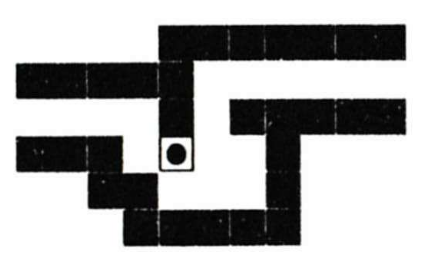
\includegraphics[width=0.3\textwidth]{images/nphard-1.png} 
    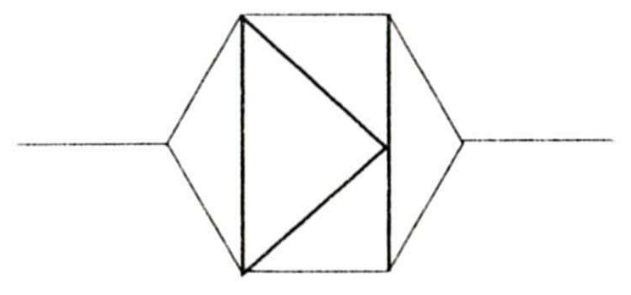
\includegraphics[width=0.3\textwidth]{images/nphard-5.png} 
    \caption{}\label{fig:nphard-1}
\end{figure}

Figure \ref{fig:nphard-1} shows a level with one entrance on the left and one exit on the right. The player can travel from the entrance to the exit by pushing the barrel (marked with a black circle) to the right and, after going through, back to the left in order to clear the path to the exit. Not only does this clear the path for the player, but it also places the barrel back on the goal position, marked with a square. However, the player cannot travel from the exit to the entrance because the player can only push the box to the left, which would block the path and render the box immobile. This structure is called a \textit{turnstile}.

\begin{figure}[h] % [h] forces the image to be placed "here"
    \centering
    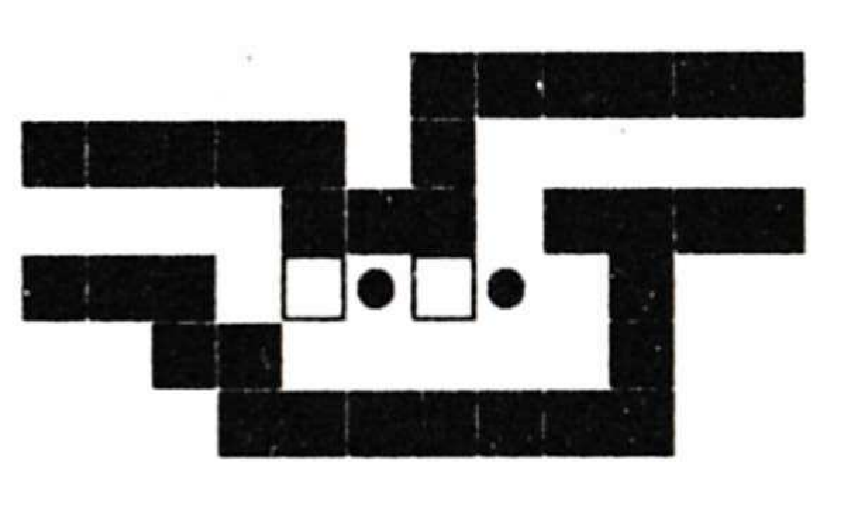
\includegraphics[width=0.3\textwidth]{images/nphard-2.png} 
    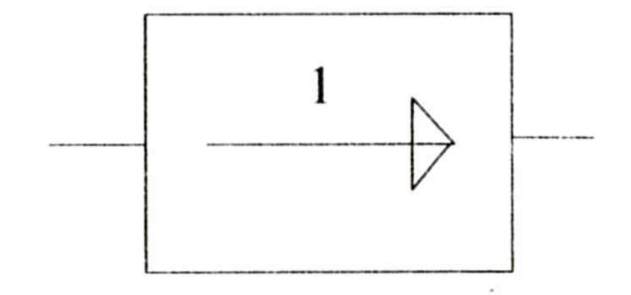
\includegraphics[width=0.3\textwidth]{images/nphard-6.png} 
    \caption{}
    \label{fig:nphard-2}
\end{figure}

Figure \ref{fig:nphard-2} shows a \textit{1-gate} that can only be traveled once by the player, and only in one direction, from left to right. This is because the left barrel needs to be pushed to the left to its goal position to be considered solved, and this action must precede the movement of the right barrel, which, after its push to the left, would prevent the left barrel from being moved. This gate can be placed in parallel to create an \textit{n-gate}, which allows traversal from left to right $n$ times.

Using a combination of $n\text{-gates}$ and $turnstiles$, we will construct the following boolean expression:
$$B(x,y,z) = (z\ \land\ \{(\neg y\ \land \neg z) \lor (\neg x\ \lor y)\})$$

\begin{figure}[h] % [h] forces the image to be placed "here"
    \centering
    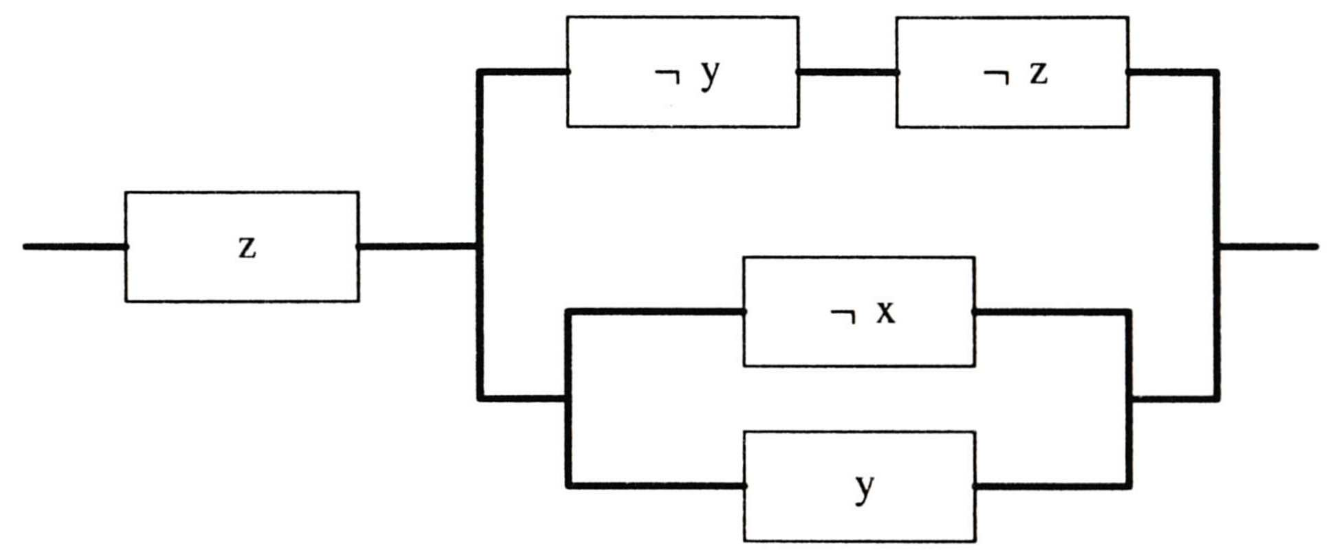
\includegraphics[width=0.8\textwidth]{images/nphard-3.png} 
    \caption{}
    \label{fig:nodegraph}
\end{figure}

The same boolean expression can be expressed as a graph of nodes (Figure \ref{fig:nodegraph}) where the player can only travel from left to right. 

For a given set of $x,y,z$, each node is traversable only if the expression inside is true. 

If the player can start from the left-end of the graph and reach the right-end of the graph, $B(x,y,z)$ is true. 

For example, if $x=0,y=0,z=1$, it would go through the nodes $z$ and $ \neg x$ to reach the right-end of the graph. 

This graph can then be recreated with the previous Sokoban level sections if we define each node as following:

\begin{figure}[h] % [h] forces the image to be placed "here"
    \centering
    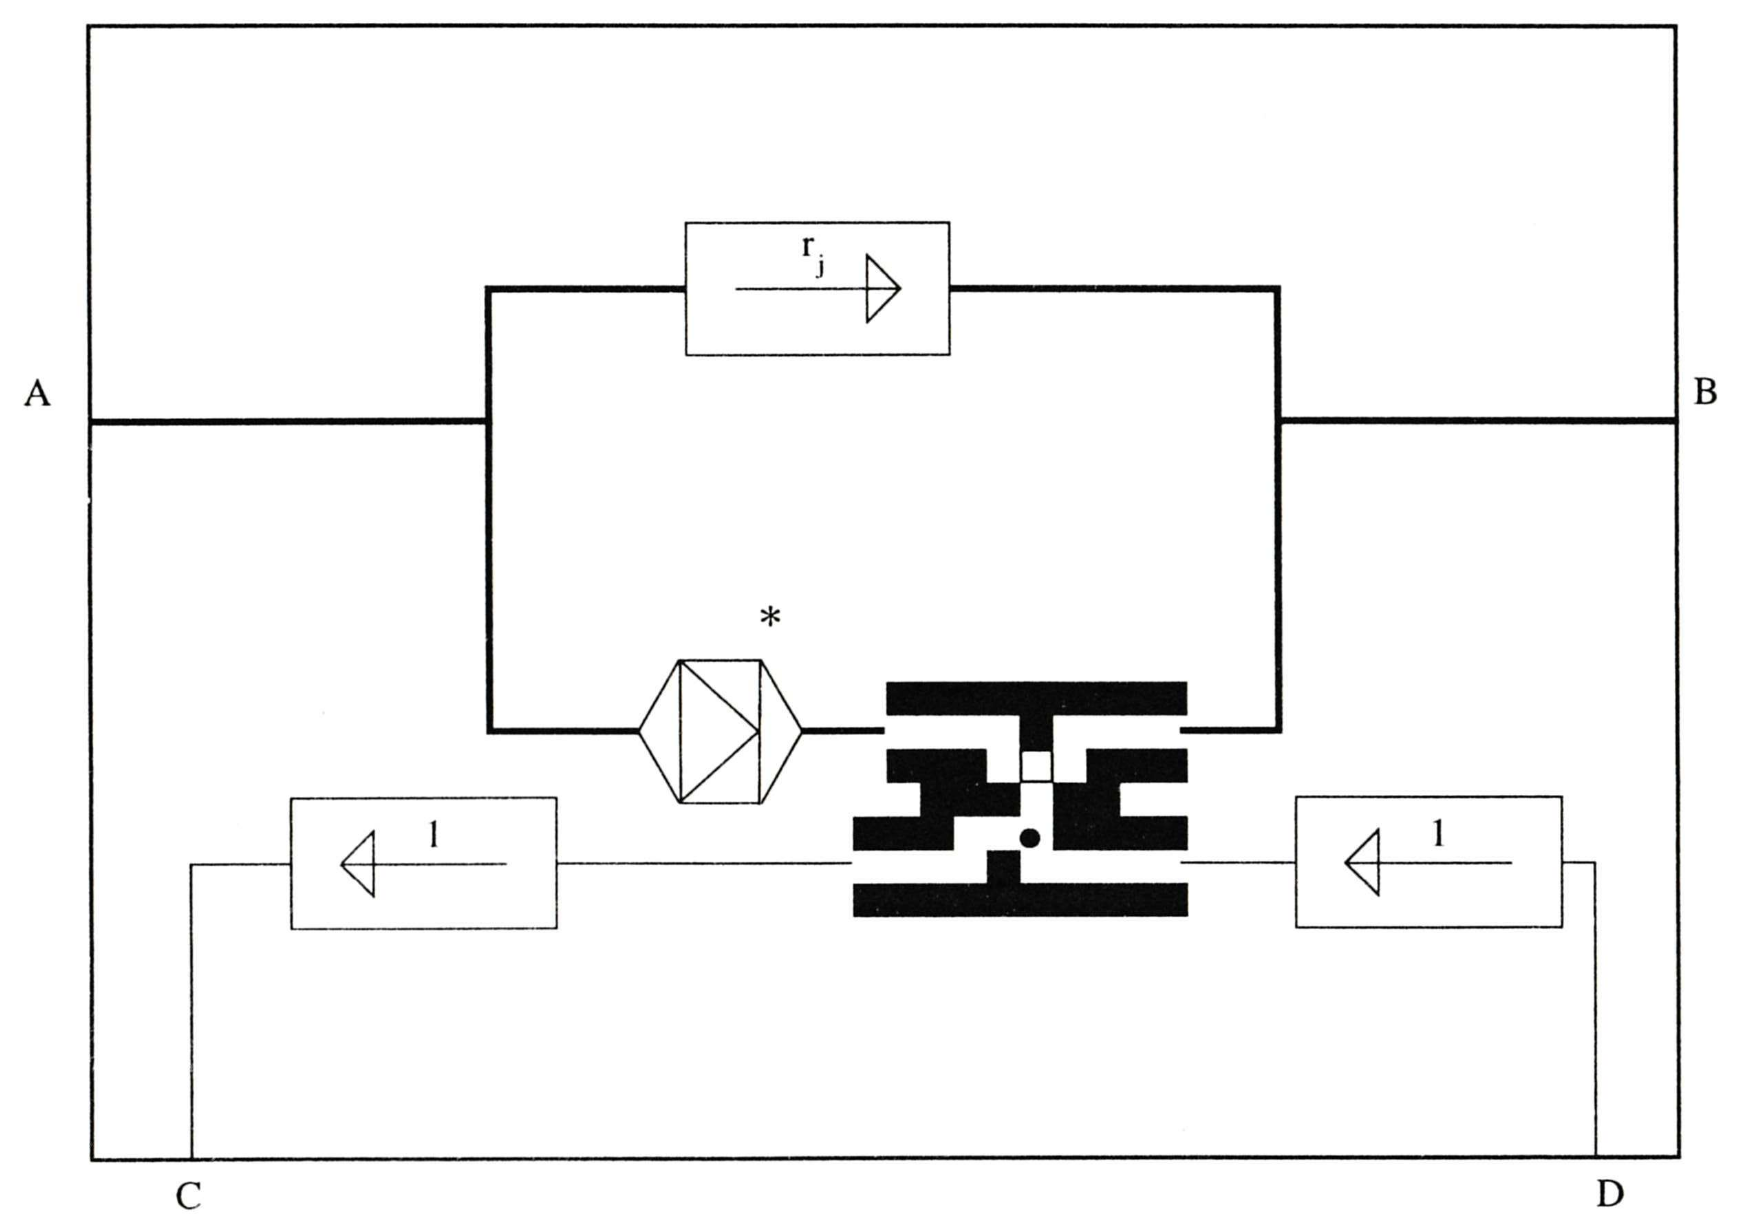
\includegraphics[width=0.8\textwidth]{images/nphard-4.png} 
    \caption{}
    \label{fig:nphard-4}
\end{figure}

The node has entrances $A,D$ and exits $B,C$. The player can traverse the node on the bold line through either the $r_j\text{-gate}$ (an $n\text{-gate}$ that can be traveled through $r_j$ times) or the $turnstile$. Notice that if the player enters $D$ and leaves through $C$, it blocks the $turnstile$ path above and forces the player to go through the $r_j\text{-gate}$ path, as the barrel will be pushed upwards into the $turnstile$ path and become stuck there. The bold path and the faint path are separate because, even though the barrel can be pushed away, it would cause the barrel to get stuck in a non-goal position. This node will be incorporated into the node graph from Figure \ref{fig:nodegraph} in a way that blocks the bold path of the $x$ node when $x=0$, blocks $\neg y$ when $y=1$, and so on.

To show that $B$ has a solution, the player has to be able to complete the node graph implemented in Sokoban shown in Figure \ref{fig:b_implementation}. (Figure \ref{fig:b_implementation} also uses a crossover implemented in Sokoban, which is omitted in this paper for brevity.)

Suppose $B(x,y,z)$ as implemented in Figure \ref{fig:b_implementation} is true (solvable with all barrels on their goal positions) and there exists a set of inputs $(x_1,x_2,\ ... , x_n)$ (which is $x,y,z$ in our expression) that makes $B$ true. With this condition, the player can solve $B$ by following the steps below:

\begin{enumerate}
    \item From `start', travel the path $x$ if $x$ is true and $\neg x$ otherwise, and so on.
    \item The player reaches P for the first time. From here, travel the bold paths using the $turnstile$ path of each node without using the $r_j\text{-gates}$, which can be done because $B$ is true. The player reaches Q.
    \item Traverse the faint paths not used in the first cycle to return to P.
    \item From P, use the bold paths to reach Q, using the $r_j\text{-gates}$ of the set of nodes that connect P to Q.
    \item The player has now fully solved the path between `start' and P. The remaining combinations of the bold paths that connect P to Q can be traveled by using the bottom bold line that has no node.
    \item After traveling through the $(r+1)\text{-gate}$ $r+1$ times, the player can place the barrel in the R section to complete the entire level.
\end{enumerate}

This demonstrates that Sokoban can successfully encode an $NP\text{-hard}$ problem and is therefore an $NP\text{-hard}$ problem itself. Readers can choose to complete Figure \ref{fig:b_implementation} by hand with the truth table below:

\begin{table}[h]
\centering
\label{tab:sokoban_logic}
\renewcommand{\arraystretch}{1.2} % Adds breathing room between rows
\begin{tabular}{ @{} ccc | ccc | cc | c | c @{} }
\toprule
$x$ & $y$ & $z$ & $\neg x$ & $\neg y$ & $\neg z$ & $\neg y \land \neg z$ & $\neg x \lor y$ & Inner Term & $B(x,y,z)$ \\
\midrule
0 & 0 & 0 & 1 & 1 & 1 & 1 & 1 & 1 & 0 \\
0 & 0 & 1 & 1 & 1 & 0 & 0 & 1 & 1 & 1 \\
0 & 1 & 0 & 1 & 0 & 1 & 0 & 1 & 1 & 0 \\
1 & 0 & 0 & 0 & 1 & 1 & 1 & 0 & 1 & 0 \\
\addlinespace % Visual break for readability
0 & 1 & 1 & 1 & 0 & 0 & 0 & 1 & 1 & 1 \\
1 & 0 & 1 & 0 & 1 & 0 & 0 & 0 & 0 & 0 \\
1 & 1 & 0 & 0 & 0 & 1 & 0 & 1 & 1 & 0 \\
\addlinespace % Visual break for readability
1 & 1 & 1 & 0 & 0 & 0 & 0 & 1 & 1 & 1 \\
\bottomrule
\end{tabular}
\caption{Truth table for the Boolean function $B(x,y,z)$}
\end{table}


